\documentclass[10pt,a4paper]{article}
\usepackage[utf8]{inputenc}
\usepackage[top=2cm,bottom=2cm,left=2cm,right=2cm]{geometry}
\usepackage{amsmath}
\usepackage{amssymb}
\usepackage{array}
\usepackage{tikz}
\usetikzlibrary{arrows.meta,calc,patterns,positioning,decorations.pathreplacing}
\usepackage{pgfplots}
\pgfplotsset{compat=1.18}
\usepackage[dvipsnames,svgnames]{xcolor}
\usepackage{hyperref}

% Anchor persamaan unik meski nomor di-reset per soal.
\newcounter{eqblock}
\newcommand{\reseteq}{%
  \stepcounter{eqblock}%
  \setcounter{equation}{0}%
  \renewcommand{\theHequation}{\arabic{eqblock}.\arabic{equation}}%
}

\pgfplotsset{
  grafik/.style={
    axis lines=middle,
    xlabel={$x$}, ylabel={$y$},
    width=7.5cm, height=6cm,
    grid=major, grid style={gray!25},
    tick label style={font=\scriptsize},
    every axis x label/.style={at={(ticklabel* cs:1)},anchor=west},
    every axis y label/.style={at={(ticklabel* cs:1)},anchor=south},
    title style={yshift=2ex},
  },
}

\title{Tugas Minggu 9 : Integral}
\author{Matematika untuk Sistem Informasi}
\date{}

\begin{document}

\maketitle

\begin{enumerate}

%===========================================================
\item Tentukan hasil dari integral berikut.
\begin{enumerate}

%-----------------------------------------------------------
\item $\displaystyle\int (x^3 + 6x)(6x^2 + 12)\, dx$

\textbf{Jawab:}
\begin{itemize}
\item \textbf{Langkah 1: Jabarkan Hasil Kali}

\reseteq
\begin{align}
(x^3 + 6x)(6x^2 + 12) &= 6x^5 + 12x^3 + 36x^3 + 72x = 6x^5 + 48x^3 + 72x
\end{align}

\item \textbf{Langkah 2: Integralkan per Suku (Kelinearan dan Aturan Pangkat)}

\reseteq
\begin{align}
\int (6x^5 + 48x^3 + 72x)\, dx &= 6 \cdot \frac{x^6}{6} + 48 \cdot \frac{x^4}{4} + 72 \cdot \frac{x^2}{2} + C \\
&= x^6 + 12x^4 + 36x^2 + C
\end{align}

\item \textbf{Langkah 3: Cek dengan Substitusi}

Misalkan $u = x^3 + 6x$, maka $du = (3x^2 + 6)\, dx$, dan $6x^2 + 12 = 2(3x^2 + 6)$:
\reseteq
\begin{align}
\int (x^3 + 6x)(6x^2 + 12)\, dx &= \int 2u\, du = u^2 + C = (x^3 + 6x)^2 + C \\
&= x^6 + 12x^4 + 36x^2 + C \quad \text{(Jabarkan kuadrat)}
\end{align}
Kedua cara memberikan hasil yang sama.
% final: x^6 + 12x^4 + 36x^2 + C
\end{itemize}

%-----------------------------------------------------------
\item $\displaystyle\int \frac{2x^6 - 3x^4 - x^3}{x^3}\, dx$

\textbf{Jawab:}
\begin{itemize}
\item \textbf{Langkah 1: Bagi Setiap Suku dengan $x^3$}

Untuk $x \neq 0$:
\reseteq
\begin{align}
\frac{2x^6 - 3x^4 - x^3}{x^3} &= \frac{2x^6}{x^3} - \frac{3x^4}{x^3} - \frac{x^3}{x^3} = 2x^3 - 3x - 1
\end{align}

\item \textbf{Langkah 2: Integralkan per Suku}

\reseteq
\begin{align}
\int (2x^3 - 3x - 1)\, dx &= 2 \cdot \frac{x^4}{4} - 3 \cdot \frac{x^2}{2} - x + C = \frac{x^4}{2} - \frac{3x^2}{2} - x + C
\end{align}
% final: \frac{x^4}{2} - \frac{3x^2}{2} - x + C
\end{itemize}

\end{enumerate}

%===========================================================
\item Diketahui
\[
\int_1^9 f(x)\, dx = -1, \qquad \int_7^9 f(x)\, dx = 5, \qquad \text{dan} \qquad \int_7^9 h(x)\, dx = 4.
\]
Tentukan:
\begin{enumerate}

%-----------------------------------------------------------
\item $\displaystyle\int_1^9 -2f(x)\, dx$

\textbf{Jawab:}
\begin{itemize}
\item \textbf{Langkah 1: Keluarkan Konstanta (Sifat Linear)}

\reseteq
\begin{align}
\int_1^9 -2f(x)\, dx &= -2\int_1^9 f(x)\, dx = -2(-1) = 2
\end{align}
% final: 2
\end{itemize}

%-----------------------------------------------------------
\item $\displaystyle\int_7^9 \bigl[2f(x) - 3h(x)\bigr]\, dx$

\textbf{Jawab:}
\begin{itemize}
\item \textbf{Langkah 1: Sifat Linear}

\reseteq
\begin{align}
\int_7^9 \bigl[2f(x) - 3h(x)\bigr]\, dx &= 2\int_7^9 f(x)\, dx - 3\int_7^9 h(x)\, dx \\
&= 2(5) - 3(4) = 10 - 12 = -2
\end{align}
% final: -2
\end{itemize}

%-----------------------------------------------------------
\item $\displaystyle\int_9^1 f(x)\, dx$

\textbf{Jawab:}
\begin{itemize}
\item \textbf{Langkah 1: Batas Ditukar}

Menukar batas atas dan batas bawah mengubah tanda integral:
\reseteq
\begin{align}
\int_9^1 f(x)\, dx &= -\int_1^9 f(x)\, dx = -(-1) = 1
\end{align}
% final: 1
\end{itemize}

%-----------------------------------------------------------
\item $\displaystyle\int_1^7 f(x)\, dx$

\textbf{Jawab:}
\begin{itemize}
\item \textbf{Langkah 1: Sifat Aditif}

Karena $1 < 7 < 9$, selang $[1, 9]$ dapat dipecah di $x = 7$:
\begin{center}
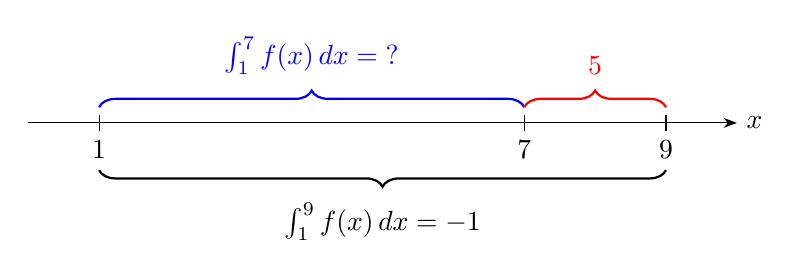
\begin{tikzpicture}[x=0.9cm]
  \draw[-{Stealth}] (0,0) -- (10,0) node[right] {$x$};
  \foreach \t in {1,7,9} {
    \draw (\t,0.1) -- (\t,-0.1) node[below] {$\t$};
  }
  \draw[decorate, decoration={brace, amplitude=6pt}, thick, blue] (1,0.2) -- (7,0.2)
    node[midway, above=8pt] {$\int_1^7 f(x)\, dx = \;?$};
  \draw[decorate, decoration={brace, amplitude=6pt}, thick, Red] (7,0.2) -- (9,0.2)
    node[midway, above=8pt] {$5$};
  \draw[decorate, decoration={brace, amplitude=6pt, mirror}, thick] (1,-0.6) -- (9,-0.6)
    node[midway, below=8pt] {$\int_1^9 f(x)\, dx = -1$};
\end{tikzpicture}
\end{center}
\reseteq
\begin{align}
\int_1^9 f(x)\, dx &= \int_1^7 f(x)\, dx + \int_7^9 f(x)\, dx
\end{align}

\item \textbf{Langkah 2: Selesaikan}

\reseteq
\begin{align}
\int_1^7 f(x)\, dx &= \int_1^9 f(x)\, dx - \int_7^9 f(x)\, dx = -1 - 5 = -6
\end{align}
% final: -6
\end{itemize}

\end{enumerate}

%===========================================================
\item Dengan menggunakan TDK I, tentukan turunan dari:
\begin{enumerate}

%-----------------------------------------------------------
\item $G(x) = \displaystyle\int_x^{x^2} \frac{t^2}{t^3 + 1}\, dt$

\textbf{Jawab:}
\begin{itemize}
\item \textbf{Langkah 1: Kenali Integran dan Batas}

$f(t) = \dfrac{t^2}{t^3 + 1}$, batas bawah $u(x) = x$ ($u' = 1$), dan batas atas $v(x) = x^2$ ($v' = 2x$).

\item \textbf{Langkah 2: Substitusikan Batas ke Integran}

\reseteq
\begin{align}
f(x^2) &= \frac{(x^2)^2}{(x^2)^3 + 1} = \frac{x^4}{x^6 + 1}, \qquad f(x) = \frac{x^2}{x^3 + 1}
\end{align}

\item \textbf{Langkah 3: Gunakan Rumus Umum TDK I}

\reseteq
\begin{align}
G'(x) &= f\bigl(v(x)\bigr) \cdot v'(x) - f\bigl(u(x)\bigr) \cdot u'(x) = \frac{x^4}{x^6 + 1} \cdot 2x - \frac{x^2}{x^3 + 1} \cdot 1 \\
&= \frac{2x^5}{x^6 + 1} - \frac{x^2}{x^3 + 1}
\end{align}
% final: G'(x) = \frac{2x^5}{x^6 + 1} - \frac{x^2}{x^3 + 1}
\end{itemize}

%-----------------------------------------------------------
\item $G(x) = \displaystyle\int_2^{x^2 + 1} \sqrt{2 + \sin t}\, dt$

\textbf{Jawab:}
\begin{itemize}
\item \textbf{Langkah 1: Kenali Integran dan Batas}

$f(t) = \sqrt{2 + \sin t}$, batas bawah $2$ (konstanta, turunannya $0$), dan batas atas $v(x) = x^2 + 1$ ($v' = 2x$).

\item \textbf{Langkah 2: Gunakan Rumus TDK I}

\reseteq
\begin{align}
G'(x) &= \sqrt{2 + \sin(x^2 + 1)} \cdot 2x - \sqrt{2 + \sin 2} \cdot 0 = 2x\sqrt{2 + \sin(x^2 + 1)}
\end{align}
% final: G'(x) = 2x\sqrt{2 + \sin(x^2 + 1)}
\end{itemize}

%-----------------------------------------------------------
\item $G(x) = \displaystyle\int_1^{x^3} \frac{1}{\sqrt{1 + t^3}}\, dt$

\textbf{Jawab:}
\begin{itemize}
\item \textbf{Langkah 1: Kenali Integran dan Batas}

$f(t) = \dfrac{1}{\sqrt{1 + t^3}}$, batas bawah $1$ (konstanta), dan batas atas $v(x) = x^3$ ($v' = 3x^2$).

\item \textbf{Langkah 2: Substitusikan Batas dan Gunakan Rumus TDK I}

\reseteq
\begin{align}
f(x^3) &= \frac{1}{\sqrt{1 + (x^3)^3}} = \frac{1}{\sqrt{1 + x^9}} \\
G'(x) &= \frac{1}{\sqrt{1 + x^9}} \cdot 3x^2 = \frac{3x^2}{\sqrt{1 + x^9}}
\end{align}
% final: G'(x) = \frac{3x^2}{\sqrt{1 + x^9}}
\end{itemize}

\end{enumerate}

%===========================================================
\item Tentukan nilai integral tentu berikut menggunakan TDK II.
\begin{enumerate}

%-----------------------------------------------------------
\item $\displaystyle\int_{-2}^{3} (x + 3)\, dx$

\textbf{Jawab:}
\begin{itemize}
\item \textbf{Langkah 1: Cari Anti Turunan}

$F(x) = \dfrac{x^2}{2} + 3x$.

\item \textbf{Langkah 2: Substitusikan Batas dan Kurangkan}

\reseteq
\begin{align}
\int_{-2}^{3} (x + 3)\, dx &= \Bigl[\frac{x^2}{2} + 3x\Bigr]_{-2}^{3} = \left(\frac{9}{2} + 9\right) - \left(\frac{4}{2} - 6\right) \\
&= \frac{27}{2} - (-4) = \frac{27}{2} + \frac{8}{2} = \frac{35}{2}
\end{align}

\item \textbf{Langkah 3: Cek dengan Luas Trapesium}

Pada $[-2, 3]$ berlaku $x + 3 \geq 0$, sehingga integral sama dengan luas trapesium dengan sisi sejajar $f(-2) = 1$ dan $f(3) = 6$, serta tinggi $5$:
\[
\frac{1 + 6}{2} \cdot 5 = \frac{35}{2}.
\]
\begin{center}
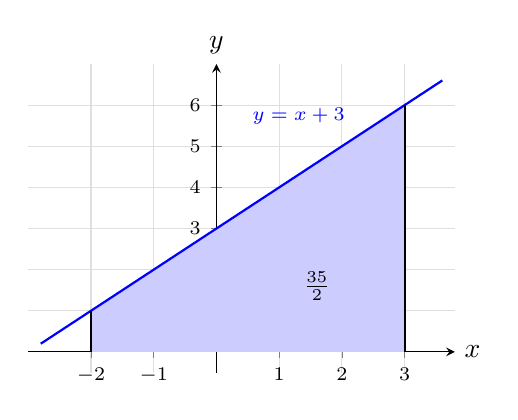
\begin{tikzpicture}
\begin{axis}[grafik, width=7cm, height=5.5cm, xmin=-3, xmax=3.8, ymin=-0.5, ymax=7, xtick={-2,-1,1,2,3}, ytick={1,2,3,4,5,6}]
  \addplot[domain=-2:3, fill=blue!20, draw=none] {x + 3} \closedcycle;
  \addplot[domain=-2.8:3.6, thick, blue] {x + 3};
  \draw[thick] (axis cs:-2,0) -- (axis cs:-2,1);
  \draw[thick] (axis cs:3,0) -- (axis cs:3,6);
  \node[font=\small] at (axis cs:1.6,1.6) {$\frac{35}{2}$};
  \node[font=\scriptsize, blue, anchor=south east] at (axis cs:2.2,5.3) {$y = x + 3$};
\end{axis}
\end{tikzpicture}
\end{center}
% final: \frac{35}{2}
\end{itemize}

%-----------------------------------------------------------
\item $\displaystyle\int_0^2 (x^2 + 1)^2\, dx$

\textbf{Jawab:}
\begin{itemize}
\item \textbf{Langkah 1: Jabarkan Integran}

$(x^2 + 1)^2 = x^4 + 2x^2 + 1$.

\item \textbf{Langkah 2: Cari Anti Turunan}

$F(x) = \dfrac{x^5}{5} + \dfrac{2x^3}{3} + x$.

\item \textbf{Langkah 3: Substitusikan Batas dan Kurangkan}

\reseteq
\begin{align}
\int_0^2 (x^4 + 2x^2 + 1)\, dx &= \Bigl[\frac{x^5}{5} + \frac{2x^3}{3} + x\Bigr]_0^2 = \left(\frac{32}{5} + \frac{16}{3} + 2\right) - 0 \\
&= \frac{96}{15} + \frac{80}{15} + \frac{30}{15} = \frac{206}{15} \quad \text{(Samakan penyebut 15)}
\end{align}
% final: \frac{206}{15}
\end{itemize}

\end{enumerate}

%===========================================================
\item Tentukan hasil dari integral berikut.
\begin{enumerate}

%-----------------------------------------------------------
\item $\displaystyle\int x^2(x^3 + 5)^9\, dx$

\textbf{Jawab:}
\begin{itemize}
\item \textbf{Langkah 1: Pilih $u$}

Misalkan $u = x^3 + 5$, maka $du = 3x^2\, dx$, sehingga $x^2\, dx = \frac{1}{3}\, du$.

\item \textbf{Langkah 2: Substitusi dan Integralkan}

\reseteq
\begin{align}
\int x^2(x^3 + 5)^9\, dx &= \frac{1}{3}\int u^9\, du = \frac{1}{3} \cdot \frac{u^{10}}{10} + C = \frac{1}{30}(x^3 + 5)^{10} + C
\end{align}
% final: \frac{1}{30}(x^3 + 5)^{10} + C
\end{itemize}

%-----------------------------------------------------------
\item $\displaystyle\int \cos(3x + 2)\, dx$

\textbf{Jawab:}
\begin{itemize}
\item \textbf{Langkah 1: Pilih $u$}

Misalkan $u = 3x + 2$, maka $du = 3\, dx$, sehingga $dx = \frac{1}{3}\, du$.

\item \textbf{Langkah 2: Substitusi dan Integralkan}

\reseteq
\begin{align}
\int \cos(3x + 2)\, dx &= \frac{1}{3}\int \cos u\, du = \frac{1}{3}\sin u + C = \frac{1}{3}\sin(3x + 2) + C
\end{align}
% final: \frac{1}{3}\sin(3x + 2) + C
\end{itemize}

%-----------------------------------------------------------
\item $\displaystyle\int 3x\sqrt{3x^2 + 7}\, dx$

\textbf{Jawab:}
\begin{itemize}
\item \textbf{Langkah 1: Pilih $u$}

Misalkan $u = 3x^2 + 7$, maka $du = 6x\, dx$, sehingga $3x\, dx = \frac{1}{2}\, du$.

\item \textbf{Langkah 2: Substitusi dan Integralkan}

\reseteq
\begin{align}
\int 3x\sqrt{3x^2 + 7}\, dx &= \frac{1}{2}\int u^{1/2}\, du = \frac{1}{2} \cdot \frac{2}{3}u^{3/2} + C = \frac{1}{3}(3x^2 + 7)^{3/2} + C
\end{align}
Bentuk lain: $\frac{1}{3}\sqrt{(3x^2 + 7)^3} + C$.
% final: \frac{1}{3}(3x^2 + 7)^{3/2} + C
\end{itemize}

%-----------------------------------------------------------
\item $\displaystyle\int_0^1 (x^2 + 2x)^2 (x + 1)\, dx$

\textbf{Jawab:}
\begin{itemize}
\item \textbf{Langkah 1: Pilih $u$ dan Sesuaikan Konstanta}

Misalkan $u = x^2 + 2x$, maka $du = (2x + 2)\, dx = 2(x + 1)\, dx$, sehingga $(x + 1)\, dx = \frac{1}{2}\, du$.

\item \textbf{Langkah 2: Ubah Batas}

Untuk $x = 0$ diperoleh $u = 0$, dan untuk $x = 1$ diperoleh $u = 1 + 2 = 3$.

\item \textbf{Langkah 3: Substitusi dan Hitung}

\reseteq
\begin{align}
\int_0^1 (x^2 + 2x)^2 (x + 1)\, dx &= \frac{1}{2}\int_0^3 u^2\, du = \frac{1}{2}\Bigl[\frac{u^3}{3}\Bigr]_0^3 = \frac{1}{2} \cdot \frac{27}{3} = \frac{9}{2}
\end{align}
% final: \frac{9}{2}
\end{itemize}

\end{enumerate}

\end{enumerate}

\end{document}
